%%%%%%%%%%%%%%%%%%%%%%%%%%%%%%%%%%%%%%%%%%%%%%%%%%%%%%%%%%%%%%%%%%%%%%%%%%%%%%%%%%%%%%%%%%%%%%%%%%%%
% NONLINEAR THEORY 
%
% 
%%%%%%%%%%%%%%%%%%%%%%%%%%%%%%%%%%%%%%%%%%%%%%%%%%%%%%%%%%%%%%%%%%%%%%%%%%%%%%%%%%%%%%%%%%%%%%%%%%%%
\chapter{Nonlinear theory}

In this chapter we extended the results of the linear stability analysis to a nonlinear analysis. Through numerical simulations, we suggest that the saturation level of the short-wave aspect ratio depends upon the aspect ratio. 

%\begin{itemize}
%\item Discuss nonlinear numerical set-up
%\item Just short wave results
%\item Scaling analysis 
%\item A few complete nonlinear simulations that capture all the dynamics.
%\item Appendix containing discussion of calculating theoretical quantities after conclusion
%\end{itemize}

\section{Set-up}
In this section we discuss some numerical tests of the code to verify that the nonlinear results are correctly resolving the samllest scales. 
In order to do a full DNS, we need to resolve the Kolmogorov scales. The Kolomogorov scale is given by (cite)
\begin{align}
\eta = \left(\frac{\nu^{3}}{\epsilon}\right)^{3}
\end{align}
where $\epsilon$ is the energy given by
\begin{align}
\epsilon \sim \frac{U^{3}}{R} 
\end{align}
where $U,R$ are the characteristic velocity and length respectively. Rewriting the Kolmogorov scale $\eta$ in terms of the Reynolds number by multipying by the characteristic length $R$, which we take to be unity as has been suggested from the linear results, to obtain
\begin{align}
\eta = \frac{1}{\Re^{3/4}}
\end{align}
For our simulations, the code seperates the horizontal and vertical resolutions, which we denote by $\Delta x$ and $\Delta z$. We want to choose the number of grid points to be such that $\Delta x \approx \Delta z$. 

To illustrate, we consider a test case that was run to determine whether or not to use $L=9$ or $L=5$ for the box size. Both have been used in practice (cite). Consider a grid with $N\times N \times n$ points, where we have explicitly seperated out the horizontal and vertical directions. Because we need to resolve the Kolmogorov scales, we have restrictions on the total number of grid points. We consider the case of $Re=2000$ and $F_{h}=0.2$. The Reynolds number tells us that that the Kolmogorov scale is
\begin{align}
\eta \sim \frac{1}{Re^{3/4}} \approx 0.003343,\qquad \Delta x \sim \eta 
\end{align}
and thus we want a grid spacing that is approximately $0.003343$. Since it is desirable for $N$ to be a power of two, if $N=1024$ we have that 
\begin{align}
\dx = \frac{L}{1024}.
\end{align}
If $L=9$ then $\dx=0.00878$ and if $L=5$ then $\dx=0.00488$. It is clear that it is more desirable to pick $L=5$ because the grid spacing is closer to the $\eta$. 

Now we need to set the vertical resolution. It is important that we have the same resolution for the vertical and horizontal so $\dx \approx \Delta z$. Since we are interested in investigating the short-wave instability the vertical scale is 
\begin{align}
H \sim \frac{2\pi}{k_{z}}.
\end{align}
In this case, the greatest growth rate occurs at the wavenumber $k_{z}=20$ and thus the vertical scale is $H=0.314$. Now setting $\Delta z \approx \dx$ for both $L=5,9$ we find that for $L=9$ if $n=32$ then $\Delta z=0.00982$ which is close to $\dx=0.00878$. If $L=5$ then if $n=64$ then $\Delta z=0.00491$ which is close to $\dx=0.00488$. Thus to resolve the Kolmogorov scale as much as possible, we should choose $L=5$ with $N=1024, n=64$over $L=9$ with $N=1024, n=32$. However when the code is actually run $L=5$ takes roughly $30.8$ hours of real time versus $19.5$ hours of real time. Additionally, due to the way the code is set-up, $L=5$ requires twice as many processors as $L=9$. Additionally, due to the way the code is set-up, $L=5$ requires twice as many processors as $L=9$ which requires more resources. Thus a trade-off must be made between running at a higher resolution but taking longer versus running at a lower resolution, in the processing potentially not resolving the Kolmogorov scale, but running faster. 

\begin{figure}
\begin{center}
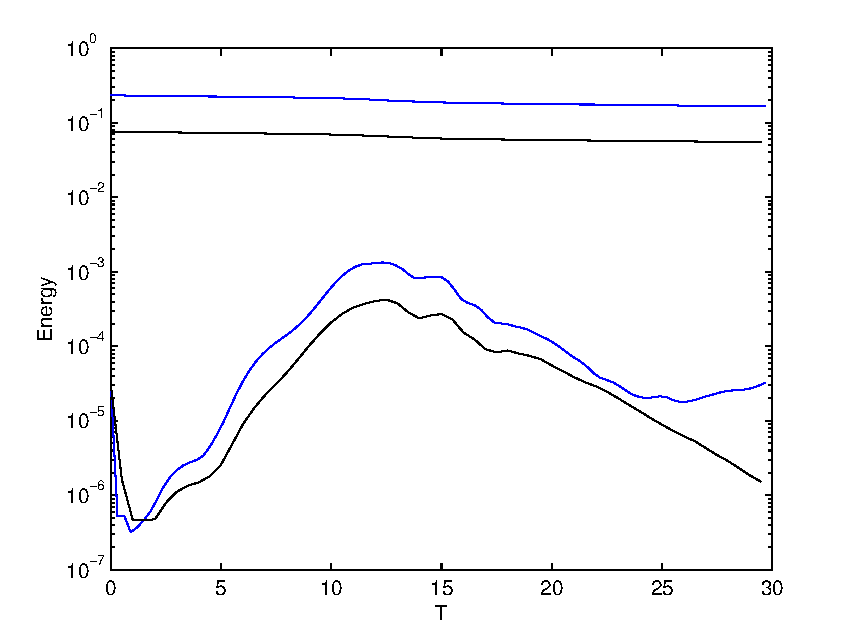
\includegraphics[width=\textwidth]{energy_test}
\caption{Time series of the potential energy (circle) and kinetic energy (star) for $L=5$ (blue) and $L=9$ (black).}
\label{test_energy}
\end{center}
\end{figure}
In Fig.~\ref{test_energy} we demonstrate two tests run that were done to determine what resolution to use. Qualitatively, both curves are very similar, with the $L=5$ curves shifted upwards by a constant. This is to be expected because by using a larger domain size, less of the domain is focused on the dipole and thus there is less energy in this dipole. When we decrease the domain size, the dipole takes up a larger percentage of the grid and thus has a larger energy. 

%\begin{figure}
%\begin{center}
%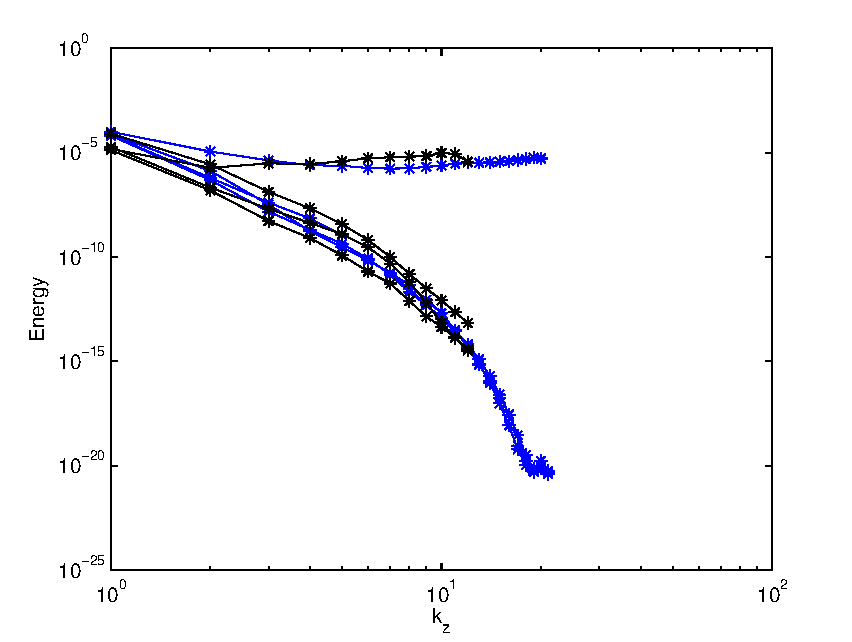
\includegraphics[width=\textwidth]{vert_spectrum_test}
%\caption{Time series of the growth rate, obtained from the derivative of the energy, for $F_{h}=0.1$ and $Re=10{,}000$. Panel (a) is $k_{z}=20$ and Panel (b) is $k_{z}60$.}
%\label{vert_spec_test}
%\end{center}
%\end{figure}
\section{Results}
The nonlinear evolution of the short-wave instability tells us how the zigzag instability and the short-wave instability interact. Investigations by Waite and Smolarkiewicz into the breakdown of the Lamb-Chaplygin dipole into turbulence and observed that the energy of the zigzag instability grew such that it became the same order of magntiude as the kinetic energy. In these simulations, no short-wave instabiltiies were observed despite having a similar growth rate. We present results that suggest that the short-wave instability saturates at a level proportional to the aspect ratio $\delta$.

To investigate the saturation level, nonlinear simulations were run with an initially small, $\epsilon=0.01$, random sinusodial perturbation of the initial density. Figure (blah) is an example of the evolution of the energy for a given set of parameters. As can be observed in this figure the saturation level occurs at roughly $T=$.  
\begin{align}
\text{saturation} = \frac{E_{3D}}{E_{2D}}
\end{align}
where we find the maximum $E_{3D}$ at later times and divide that time by the kinetic energy. 

\begin{figure}
\begin{center}
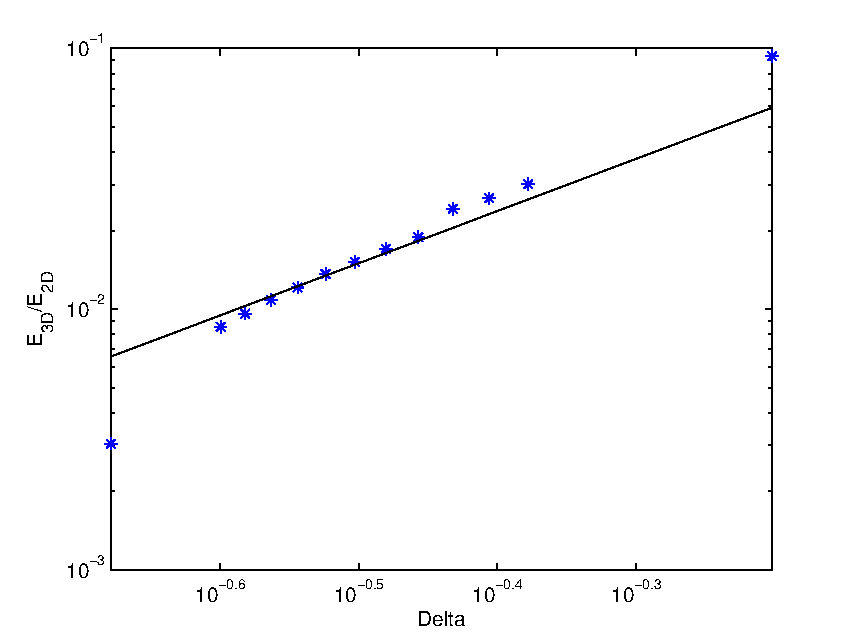
\includegraphics[width=\textwidth]{re2000_fh02_saturations} 
\caption{Saturation levels for a range of aspect ratios for $Re=2000$ and $F_{h}=0.2$.}
\label{re2000sat}
\end{center}
\end{figure}
\begin{figure}
\begin{center}
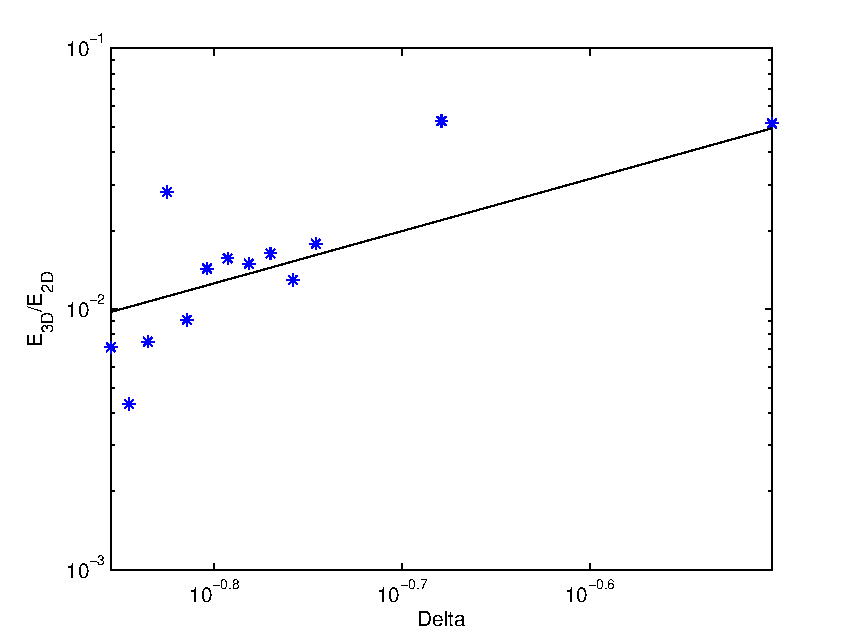
\includegraphics[width=\textwidth]{re5000_fh02_saturations} 
\caption{Saturation levels for a range of aspect ratios for $Re=5000$ and $F_{h}=0.2$. }
\label{re5000sat}
\end{center}
\end{figure}
Fig.~\ref{re2000sat} and Fig.~\ref{re5000sat} demonstrate the saturation level for $F_{h}=0.2$ and $Re=2000,5000$ respectively. The reference line is a slope of 2. In Fig.~\ref{re5000sat} there is some variation in the data points as there is no clear saturation level. Fig blah demonstrates an example of this. From these curves, it suggests that  
\begin{align}
\frac{E_{3Dsat}}{E_{2Dsat}} \sim \delta^{2}.
\end{align}
This scaling suggests that as the aspect ratio gets smaller, the saturation level decreases. 

The scaling suggested has a theoretical backing. In investigations by Ngan, et al \cite{ngan2005} into quasi-two dimensional turbulence, they determined that the saturation level of a perturbation depended linearly upon the aspect ratio. We review their derivation. Ngan et. al \cite{ngan2005} consider quasi-two dimensional turbulence, which they define to be the three-dimesionalisation of a two-dimensional flow. The study of such flows are motivated by geophysical applications were aspects ratios range from $\delta\sim 0.01-0.1$\cite{ngan2005}. 

Ngan et al. now consider a simple scaling analysis \cite{ngan2005}. Initially the time scales of the 2D base flow is long compared to that of the 3D base flow. In our results, we verify this. In figure blah note that the time scale of the 2D perturabtion, here the top line, is constant while the timescale of the 3D flow is much shorter, which is exemplified by the change that the 3D perturbation goes through over the first 20 or seconds. However once the 3D perturbation saturates, it stops growing and its timescale becomes similar to that of the 2D flowa.  Now consider the following timescales for these flows \cite{ngan2005} as
\begin{align}
T_{2D} = \frac{U}{L},\qquad T_{3D} =\frac{u}{H}
\end{align}
where $U$ is the characteristic velocity of the 2D flow and $u$ is the characteristic velocity. Thus at saturation $T_{2D}\sim T_{3D}$ and thus we have that
\begin{align}
\frac{U}{L}\sim\frac{u}{H} \Rightarrow \frac{u}{U} \sim \frac{H}{L} = \delta .
\end{align}
However we are considering the energy and thus we would have to square both sides to get the energy resulting in
\begin{align}
\frac{E_{2D}}{E_{3D}} \sim \delta^{2}
\end{align}
which is the result suggested by Figs.~\ref{re2000sat} and Fig.~\ref{re5000sat}. Thus, the short-wave instability, despite having a similar growth rate to that of the zigzag instability, is saturated at a level proportional to the aspect ratio of the flow, which in stratified flows, is small. 

%Furthermore, in the scaling analysis derived in the previous chapter, if $\delta < F_{h} \ll 1$ then the startification 


%To determine this linear relationship, they consider the following flow
%\begin{align}
%\bm{v}(x,y,z,t) = \bm{U}(x,y,t)+\bm{u}(x,y,z,t)
%\end{align}
%where $\bm{U}$ is a 2D base flow that satisfies the 2D Navier-Stokes equations and $\bm{u}$ is a 3D perturbation. 
